Mitä on web-palvelut?

Arkkitehtuureja? n-tier? Komponentit?

Pitäisikö tämän web-palvelukappaleen olla vasta tunnistautumisen jälkeen, niin voisi olla kappale tunnistautuminen web-palveluissa vai tämä vain itsenäinen web-palvelukappale ja tuohon tunnistautumiseen (ja sen ongelmiin) pureudutaan sitten neloskappaleessa.

Miten käyttäjädataa onko käsitelty ja käsitellään. Kehitys paikallisesti käytetyistä tiedostopohjaisista systeemeistä kohti tietokantoja ja asiaan räätälöihin palveluihin (LDAP). LDAP oleelisin, mutta tutkimuksen kannalta abstraktointi on tärkeä juttu.

Johdanto puoli sivua, alaluvut 0.5-1 sivu.
\subsection{Historia}
WWW:n, ja erityisesti WWW:n edeltäjän Gopherin, sivustot olivat alkujaan lähinnä staattisia dokumentteja, jotka oli linkitetty toisiinsa. Dokumentit muodostivat erillisia arkistoja esimerkiksi tutkijoiden käyttöön. Ajan kuluessa tuli tarpeelliseksi tehdä sivustoja, jotka reagoivat käyttäjän syötteeseen ja toimivat dynaamisesti käyttäjän syötteen mukaan.

Vuonna 1993 esitelty Common Gateway Interface (CGI) on standardi, jolla voidaan ajaa ohjelmia web-sivujen kautta UNIX-ympäristössä \cite{rfc3875}. Tyypillisesti CGI:llä ajettavat ohjelmat ovat itsenäisiä ja ne on kirjoitettu jollain skriptikielellä esimerkiksi Perlillä tai PHP:lla. Skripti saa parametrina käyttäjän lähettämät syötteet ja muodostaa sen perusteella käyttäjälle näkyvän HTML-sivun. Ajan kuluessa CGI-ohjelmat alkoivat kasvaa ja niiden arkkitehtuuri monimutkaistua, kun esimerkiksi niissä alettiin käyttää tietokantoja.

CGI-ohjelmien kasvun lisäksi myös niiden suoritukseen vaadittava ajoympäristö alkoi kasvaa ja muodostaa ongelmia CGI:n käytölle. CGI käynnistää suoritettavan prosessin jokaisen sivupyynnön yhteydessä, mikä voi olla hidasta, jos prosessi esimerkiksi lataa muistiin paljon dataa. Erityisesti 1990-luvulla Sunin kehittämä Java-kieli, joka saavutti suosiota web-kehittäjien keskuudessa, oli merkittävässä roolissa 1990-luvun lopun web-kehityksessä \cite{uml}.

Javan web-käyttöön suunniteltu Enterprise Edition (J2EE) käyttää Servlet-tekniikkaa, joka laajentaa perinteisen web-palvelimen toimintaa. Servlet-ohjelmia ei siis käynnistetä erillisestä web-palvelimesta, vaan se suoritetaan web-palvelimen sisällä. Käyttäjän pyynnön saatuaan web-palvelin (esimerkiksi Apache Tomcat) ohjaa pyynnön Java Servetille, joka käsiteltyään sen, palauttaa vastauksen web-palvelimelle, joka näyttää sivun käyttäjälle. Web-palvelin pitää siis Java-prosessia kokoajan käynnissä ja ympäristöä ei tarvitse käynnistää jokaisen käyttäjän pyynnön yhteydessä uudestaan. Servlet-tekniikan avulla voidaan tehostaa resurssien jakamista useamman pyynnön kesken, tehdä transaktioimalleja, muuttaa käyttäjäohjelman tilaa ja hallita web-sovelluksia etänä \cite{uml}. Eri kielille on toteutettu myös omia, Javan Servlettiä muistuttavia, web-palvelimia, esimerkiksi Ruby on Rails web-ohjelmointikehys tarjoaa oletuksena Rubyyn sisäänrakennetun WEBrick web-palvelimen, joka käynnistää ympäristön ja ohjaa pyynnöt oikeille Ruby on Rails -luokille \cite{ruby2011agile}. Kuvassa \ref{servlet} on kuvattu yksittäisen sivupyynnön kulkua Java Servlet-palvelimessa.

\begin{figure}[ht]
\centering
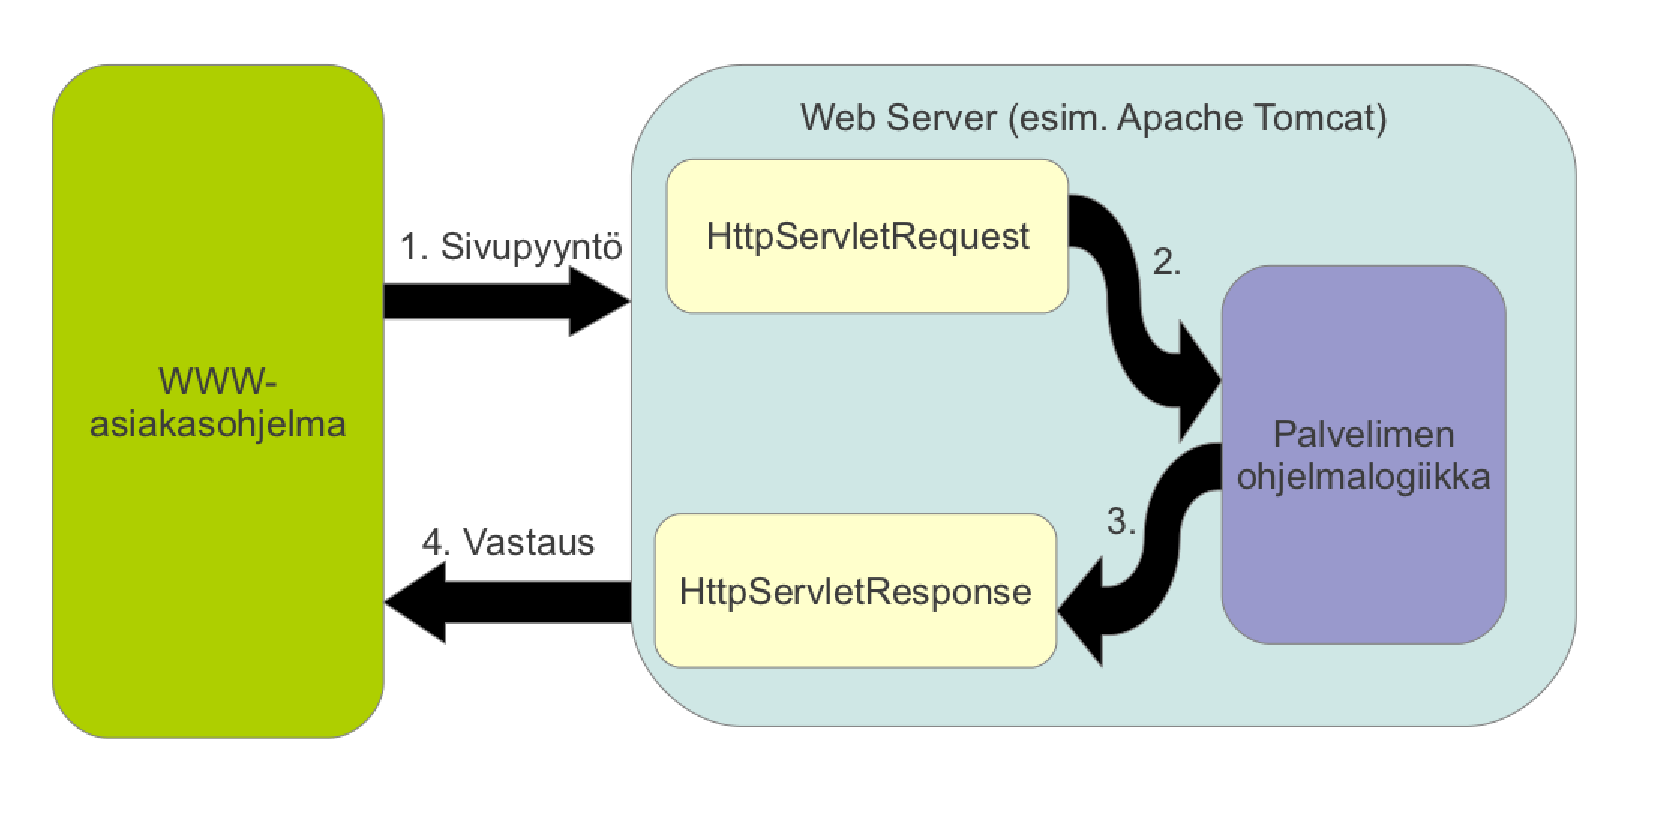
\includegraphics[width=\textwidth]{web/servlet.eps}
\caption{Kontrollin kulku Java Servlet-palvelimessa}%
\label{servlet}
\end{figure}

Servletien jälkeen paljon suosiota on saanut CGI:stä kehittynyt FastCGI-protokolla, joka korjaa CGI:ssä havaittuja puutteita \cite{fastcgi}. Web-palvelin ei käynnistä jokaista pyyntöä kohti uutta prosessia, vaan pyynnöt lähetetään ja vastaanotetaan pistokkeen (socket) avulla palvelimella suoritettavalle prosessille. FastCGI-ohjelmat voivat olla myös hajautettu eri palvelimille, jolloin pyyntöjen välitykseen käytetään TCP-yhteyttä. FastCGI:tä voidaan käyttää minkä tahansa kielen kanssa, joka tukee pistokkeiden käyttöä. Näin ollen se on varteenotettava tekniikka, koska ohjelmointikieli ei ole rajattu vain Javaan, vaan käytössä on Javan lisäksi koko kielien kirjo (esimerkiksi PHP, Python ja Ruby).

Tiivistetysti web-sovellusten historiasta voidaan sanoa, että niistä on tullut itsenäisiä ohjelmia, jotka pyörivät jatkuvasti palvelimella. Ohjelmat saavat kontrollin web-palvelimelta, joko laajentamalla web-palvelimen toimintaa (Servlet, WEBrick yms) tai pistokkeiden avulla (FastCGI). Web-sovellukset tuottavat käyttäjän syötteen ja web-sovelluksen sen hetkisen tilan mukaan käyttäjälle dynaamisen HTML tms muotoisen sivun. Seuraavissa kappaleissa pureudutaan web-sovellusten arkkitehtuuriin ja tutkitaan niiden kehitystä.
\subsection{Palvelinarkkitehtuurit}
Palvelinten yleinen arkkitehtuuri. Tietokantasovellus, sovellus yms. Ehkä vähän laajemmin kuin pelkästään palvelinten arkkitehtuurit, eli käyttäjä selaimineen mukaan. Miten kontrolli menee järjestelmässä, kun käyttäjä pyytää sivua x.

\subsection{Palveluperustaiset web-sovellukset}
Perus arkkitehtuurissa oleva sovellus pilkotaan autonomisiin kokonaisuuksiin, jotka juttelee keskenään web service -rajapintojen kautta.

tässä kai voisi kertoa kehityksen perus server-client moskasta kohti javascriptillä toteutettavia DOM-virityksiä

Erityisesti tärkeää kertoa, että käyttöliittymä ja data erotetaan toisistaan: käyttöliittymä rakennetaan javascriptillä (tai flashilla, silverlightilla whatever) ja erilliset palvelut tarjoavat sitten json/xml-dataa, jota tuo käyttöliittymä visualisoi. Gradun ongelma onkin juuri tässä: miten toteuttaa käyttöliittymä, jossa javascript hakee dataa erilaisista datalähteistä ja käyttäjä pystytään tunnistamaan näissä eri datalähteissä. Tuskin tämä kuuluu web-palveluiden historia-kappaleeseen, mutta tämän kappaleen tarkoitus on kertoa lukijalle, että tällaisia ne web-palvelut nykyään on. Eli n-tier on tässä nyt jotenkin läsnä.
\subsection{Yhteenveto}
Keskitetyn tunnistautumispalvelun käyttö on perusteltua, jos ympäristössä on useita käyttäjän tunnistamista vaativia web-sovelluksia. Tunnistautumispalvelun käytöllä ehkäistään käyttäjätietojen kopiointiin liittyviä synkronointiongelmia, kun käyttäjädata on keskitetty yhteen paikkaan. Erityisesti arkaluontoinen data, kuten salasanatiivisteet, kannattaa keskittää, jolloin ne eivät päädy vääriin käsiin yksittäisiin web-sovelluksiin kohdistuneiden tietomurtojen yhteydessä.

Tunnistautumispalvelu mahdollistaa myös muiden kuin järjestelmän ylläpitäjien tuottamien sovellusten käytön organisaation sisäisillä käyttäjätunnuksilla. Käyttämällä luotettavaksi todettuja rajapintoja, voi ylläpito antaa kolmannen osapuolen toteuttamalle web-sovellukselle oikeuden käyttää tunnistautumispalvelua käyttäjän tunnistamiseen. Tällöin käyttäjä ohjataan tunnistautumispalveluun tunnistamisen ajaksi ja web-sovellus saa vain pääsyvaltuuden, jolla sovellus voi hakea käyttäjän tiedot. Käyttäjän tunnistetiedot eivät tule missään vaiheessa tunnistamista tarvitsevan web-sovelluksen tietoon. Näin ollen esimerkiksi Facebook-tunnuksilla voi kirjautua useaan web-sovellukseen, vaikka Facebookilla ei ole tarkkaa tietoa sovelluksien sisäisestä toimintalogiikasta.

Tutkielmassa esitellyn Kapsi ry:n hallintatyökalujen tapauksessa palvelu tullaan toteuttamaan Django-sovelluskehyksellä, mutta myös valmiita toteutuksia on olemassa eri intranet-ympäristöihin. Teknologivalinta tulee tehdä sovellusympäristön mukaan, eikä yksi ratkaisu sovi kaikkiin ympäristöihin. Web-sovelluksen ja tunnistautumispalvelun välinen rajapinta pitää huolen palveluiden yhteensopivuudesta. Rajapinnoiksi on valittavissa useita eri protokollia, kuten Web Services -standardin SAML tai avoimen lähdekoodin yhteisössä syntyneet OpenID ja OAuth. Protokollien käyttö rinnakkain on myös mahdollista, jolloin tunnistautuminen voidaan tehdä esimerkiksi SAML- tai OAuth-protokollalla riippuen web-sovelluksesta.

Tunnistautumiseen liittyvien tehtävien erottaminen yksittäisiltä web-sovelluksilta erillisen palvelun tehtäväksi on palvelusuuntauneiden arkkitehtuurien periaatteiden mukaista. Tällaisten arkkitehtuurien mukaan toteutetuissa sovellusympäristöissä jokaisella web-sovelluksella on oma tarkasti määritelty tehtävä. Kun arkkitehtuurissa on oma palvelu tunnistautumiselle, on pienten yksittäisten komponenttien toteutus helpompaa, koska jokaisen komponentin kohdalla ei tarvitse huolehtia tunnistautumisen toteutuksesta.

Web-sovelluksen ja tunnistamisen erottaminen toisistaan mahdollistaa myös tunnistautumisen tehostamisen ilman muutoksia web-sovellusten toimintaan. Järjestelmässä voidaan ottaa salasanan lisäksi käyttöön toiseen tekijään perustuva tunnistaminen, jolloin esimerkiksi käyttäjän täytyy salasanan lisäksi syöttää matkapuhelimeen lähetetty tunnistekoodi. Web-sovelluksen ja tunnistautumispalvelun välinen rajapinta ei tässä tapauksessa muutu, joten tunnistamisen parantaminen ei edellytä web-sovelluksien muuttamista.

Keskitetyn pääsynvalvonnan toteuttaminen tutkielmassa kuvatuilla periaatteilla on mahdollista. Tällöin tiedot käyttäjien pääsyoikeuksista ympäristön sisällä ovat yhdessä paikassa, joka helpottaa niiden hallinnointia. Esimerkiksi henkilön siirtyessä tehtävästä toiseen, voidaan hänen pääsyvaltuudet muuttaa samasta paikasta. Pääsynvalvontaan voidaan käyttää esimerkiksi tutkielmassa esiteltyjä SAML- tai OAuth-protokollia.

Käyttäjän tunnistamista vaativissa web-sovelluksissa käyttäjän tunnistaminen kannattaa toteuttaa erillisenä komponenttina. Käytettyjen teknologioiden suhteen valinta täytyy tehdä web-sovellusympäristön mukaan, koska kaikkiin ympäristöihin sopivaa ratkaisua ei ole. Tässä tutkielmassa esitellyt periaatteet ovat kuitenkin sovellettavissa eri teknologioita käytettäessä.